\documentclass[journal]{IEEEtran}
\usepackage[a5paper, margin=10mm, onecolumn]{geometry}
\usepackage{lmodern}
\usepackage{tfrupee}
\setlength{\headheight}{1cm}
\setlength{\headsep}{0mm}

\usepackage{gvv-book}
\usepackage{gvv}
\usepackage{cite}
\usepackage{amsmath,amssymb,amsfonts,amsthm}
\usepackage{algorithmic}
\usepackage{graphicx}
\usepackage{textcomp}
\usepackage{xcolor}
\usepackage{txfonts}
\usepackage{listings}
\usepackage{enumitem}
\usepackage{mathtools}
\usepackage{gensymb}
\usepackage{comment}
\usepackage[breaklinks=true]{hyperref}
\usepackage{tkz-euclide}
\usepackage{listings}
\def\inputGnumericTable{}
\usepackage[latin1]{inputenc}
\usepackage{color}
\usepackage{array}
\usepackage{longtable}
\usepackage{calc}
\usepackage{multirow}
\usepackage{hhline}
\usepackage{ifthen}
\usepackage{lscape}
\usepackage{xparse}

\bibliographystyle{IEEEtran}

\title{12.472}
\author{EE25BTECH11043 - Nishid Khandagre}

\begin{document}
\maketitle

\renewcommand{\thefigure}{\theenumi}
\renewcommand{\thetable}{\theenumi}

\numberwithin{equation}{enumi}
\numberwithin{figure}{enumi}

\textbf{Question}:
A rigid ball of weight 100 N is suspended with the help of a string. The ball is pulled by a horizontal force F such that the string makes an angle of 30$^\circ$ with the vertical. The magnitude of force F (in N) is 

\begin{figure}[H]
\centering
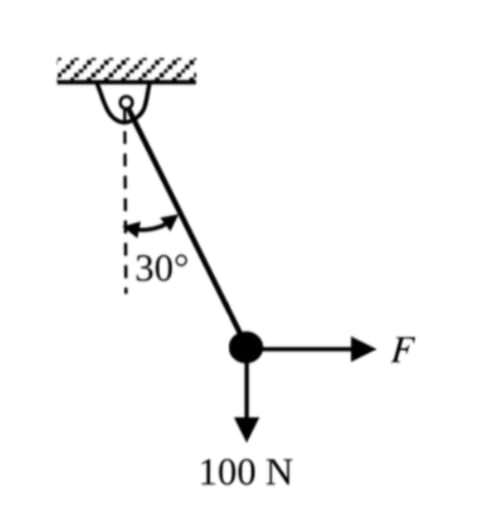
\includegraphics[width=0.4\columnwidth]{fig.jpg}
\caption{}
\label{fig:2}
\end{figure}

\textbf{Solution: }
Let $T$ be the tension in the string and $F$ the horizontal force.
Equilibrium of the ball gives the linear system:
\begin{align}
T\sin 30^\circ - F = 0, \\
T\cos 30^\circ - 100 = 0.
\end{align}
\begin{align}
\frac{1}{2}T - F &= 0, \\
\frac{\sqrt3}{2}T &= 100.
\end{align}
Writing this in matrix form $\vec{A}\vec{x}=\vec{b}$ with $\vec{x}=\myvec{T \\ F}$:
\begin{align}
\myvec{
\frac12 & -1 \\
\frac{\sqrt3}{2} & 0
}
\myvec{T \\ F}
=
\myvec{0 \\ 100}
\end{align}
Augmented matrix:
\begin{align}
\myvec{
\frac12 & -1 & \vrule & 0 \\
\frac{\sqrt3}{2} & 0 & \vrule & 100
}
\end{align}
$R_1 \rightarrow 2R_1$,$R_2 \rightarrow 2R_2$
\begin{align}
\myvec{
1 & -2 & \vrule & 0 \\
\sqrt3 & 0 & \vrule & 200
}
\end{align}
$R_2 \rightarrow R_2 - \sqrt3 R_1$:
\begin{align}
\myvec{
1 & -2 & \vrule & 0 \\
0 & 2\sqrt3 & \vrule & 200
}
\end{align}
From the second row:
\begin{align}
2\sqrt3 F &= 200 \\
F &= \frac{100}{\sqrt3}.
\end{align}
Thus, the magnitude of force $F$ is:
\begin{align}
F = \frac{100}{\sqrt3} \text{ N}.
\end{align}
Numerically,
$F \approx 57.7 \text{ N}$.

\end{document}
